\documentclass[11pt,preprint]{aastex_nofoot}
%Following line instructs TeXShop to use latex + ghostscript:
%!TEX TS-program = latex
%\documentclass[12pt]{article}
%\documentclass{/Users/adam/papers/latexfiles/emulateapj}
%\documentclass{/Users/adam/papers/latexfiles/emulateapj}
%\usepackage{/Users/adam/papers/latexfiles/emulateapj5}
%\usepackage{/Users/adam/papers/latexfiles/deluxetable}

%\special{! /pdfmark 
%            [/View [/XYZ null null 1]  % unspecified x and y offset, 100% zoom
%             /Page 1
%             /PageModehttps://www.sharelatex.com/4759396695vhbmwsvkbydp /UseThumbs % /UseNone /UserOutlines /UseThumbs /FullScreen
%            /DOCVIEW pdfmark 
%            }

\usepackage[utf8]{inputenc}
\usepackage{natbib}  % Requires natbib.sty, available from http://ads.harvard.edu/pubs/bibtex/astronat/
\usepackage{rotating}
\usepackage{savesym}
\savesymbol{singlespace}
\savesymbol{doublespace}
\usepackage{wrapfig}
\usepackage{setspace}
\usepackage{xspace}
\usepackage{color}
\usepackage{multicol}
\usepackage{mdframed}
%\citestyle{aa}  % (Author YYYY) references instead of (Author, YYYY)
%\bibliographystyle{/Users/adam/papers/latexfiles/apj_w_etal}
%\bibliographystyle{/Users/adam/papers/latexfiles/apj_w_etal_3auth}
\newcommand{\red}[1]{\textcolor{red}{#1}}
\newcommand{\todo}[1]{\textcolor{red}{#1}}
\usepackage{enumitem}
\setlist{nolistsep}
\setlist{noitemsep}
%\setlist{nosep}
%\setlist{nopartopsep}
%\setlist{noparbottomsep}
\usepackage[compact]{titlesec}
\titlespacing{\section}{0pt}{8pt}{0pt}


%%% this achieves the holy grail of 1 in margins all around!!! %%%
	%%%%%%%%%%%%%%%%%%%%%%%%%%%%%%
%	\oddsidemargin  0.0in
%	\evensidemargin 0.0in
%	\textwidth      7in
%	\headheight     0.0in
%	\topmargin      1.00in
%	\textheight=9in
	%%%%%%%%%%%%%%%%%%%%%%%%%%%%%%


% some macros that will probably be useful...
\newcommand{\paa}{Pa\ensuremath{\alpha}}
\newcommand{\brg}{Br\ensuremath{\gamma}}
\newcommand{\msun}{\ensuremath{M_{\odot}}\xspace}			%  Msun
\newcommand{\lsun}{\ensuremath{L_{\odot}}\xspace}			%  Lsun
\newcommand{\lbol}{\ensuremath{L_{\mathrm{bol}}}}	%  Lbol
\newcommand{\ks}{K\ensuremath{_{\mathrm{s}}}}		%  Ks
\newcommand{\hh}{\ensuremath{\textrm{H}_{2}}\xspace}			%  H2
\newcommand{\formaldehyde}{\ensuremath{\textrm{H}_2\textrm{CO}}\xspace}
\newcommand{\formaldehydeIso}{\ensuremath{\textrm{H}_2~^{13}\textrm{CO}}\xspace}
\newcommand{\methanol}{\ensuremath{\textrm{CH}_3\textrm{OH}}\xspace}
\newcommand{\ortho}{\ensuremath{\textrm{o-H}_2\textrm{CO}}}
\newcommand{\oneone}{\ensuremath{1_{10}-1_{11}}\xspace}
\newcommand{\twotwo}{\ensuremath{2_{11}-2_{12}}\xspace}
\newcommand{\threethree}{\ensuremath{3_{12}-3_{13}}\xspace}
\newcommand{\threeohthree}{\ensuremath{3_{03}-2_{02}}\xspace}
\newcommand{\threetwotwo}{\ensuremath{3_{22}-2_{21}}\xspace}
\newcommand{\threetwoone}{\ensuremath{3_{21}-2_{20}}\xspace}
\newcommand{\JKaKc}{\ensuremath{J_{K_a K_c}}}
\newcommand{\water}{H$_{2}$O}		%  H2O
\newcommand{\feii}{\ion{Fe}{2}}		%  FeII
\newcommand{\kms}{\textrm{km~s}\ensuremath{^{-1}}\xspace}	%  km s-1
\newcommand{\sqcm}{cm$^{2}$\xspace}		%  cm^2
\newcommand{\percc}{\ensuremath{\textrm{cm}^{-3}}\xspace}
\newcommand{\persc}{\ensuremath{\textrm{cm}^{-2}}\xspace}
\newcommand{\persr}{\ensuremath{\textrm{sr}^{-1}}\xspace}
\newcommand{\peryr}{\ensuremath{\textrm{yr}^{-1}}\xspace}
\newcommand{\perkmspc}{\textrm{per~km~s}\ensuremath{^{-1}}\textrm{pc}\ensuremath{^{-1}}\xspace}	%  km s-1 pc-1
\newcommand{\um}{\ensuremath{\mu m}\xspace}    % micron
\newcommand{\mum}{$\mu$m}
\newcommand{\htwo}{\ensuremath{\textrm{H}_2}}    % micron
\newcommand{\Htwo}{\ensuremath{\textrm{H}_2}}    % micron
\newcommand{\HtwoO}{\ensuremath{\textrm{H}_2\textrm{O}}}    % micron
\newcommand{\htwoo}{\ensuremath{\textrm{H}_2\textrm{O}}}    % micron
\newcommand{\ha}{\ensuremath{\textrm{H}\alpha}}
\newcommand{\hb}{\ensuremath{\textrm{H}\beta}}
%\newcommand{\so}{ SO~(5~6)-(4~5) }
\newcommand{\regone}{Sh~2-201}
\newcommand{\regtwo}{AFGL~4029}
\newcommand{\regthree}{LW Cas Nebula}
\newcommand{\regfour}{IC 1848}
\newcommand{\regfive}{W5 NW}
\newcommand{\regsix}{SFO 11}
\newcommand{\so}{ SO~\ensuremath{5_6-4_5} }
\newcommand{\ammonia}{NH\ensuremath{_3}\xspace}
\newcommand{\region}{W5}
\newcommand{\twelveco}{\ensuremath{^{12}\textrm{CO}}}
\newcommand{\thirteenco}{\ensuremath{^{13}\textrm{CO}}}
\newcommand{\ceighteeno}{\ensuremath{\textrm{C}^{18}\textrm{O}}}
\def\ee#1{\ensuremath{\times10^{#1}}}
\newcommand{\degree}{\ensuremath{^{\circ}}}
\newcommand{\lowirac}{800}
\newcommand{\highirac}{8000}
\newcommand{\lowmips}{600}
\newcommand{\highmips}{5000}
\newcommand{\perbeam}{\ensuremath{\textrm{beam}^{-1}}}
\newcommand{\uchii}{UC\textsc{hii}\xspace}
\newcommand{\UCHII}{UC\textsc{hii}\xspace}
\newcommand{\hchii}{HC\textsc{hii}\xspace}
\newcommand{\hii}{H{\sc ii}\xspace}
\newcommand{\hi}{H{\sc i}\xspace}
\newcommand{\Hii}{H{\sc ii}\xspace}
\newcommand{\HII}{H{\sc ii}\xspace}
\newcommand\arcdeg{\mbox{$^\circ$}\xspace} 
\newcommand\arcmin{\mbox{$^\prime$}\xspace} 
\newcommand\arcsec{\mbox{$^{\prime\prime}$}\xspace} 
\newcommand{\helv}{\fontfamily{phv}\selectfont}
\newcommand{\MUSTANG}{\textsc{MUSTANG-2}\xspace}

%\newcommand{\arcmin}{'}

\def\Figure#1#2#3#4#5{
\begin{figure*}[htp]
\epsscale{#4}
\includegraphics[scale=#4,angle=#5]{#1}
\caption{#2}
\label{#3}
\end{figure*}
}

\def\SubFigure#1#2#3#4#5{
\begin{figure*}[htp]
\addtocounter{figure}{-1}
\epsscale{#4}
\includegraphics[angle=#5]{#1}
\caption{#2}
\label{#3}
\end{figure*}
}

\def\FigureTwo#1#2#3#4#5{
\begin{figure*}[htp]
\epsscale{#5}
\plottwo{#1}{#2}
\caption{#3}
\label{#4}
\end{figure*}
}

\def\SubFigureTwo#1#2#3#4#5{
\begin{figure*}[htp]
\addtocounter{figure}{-1}
\epsscale{#5}
\plottwo{#1}{#2}
\caption{#3}
\label{#4}
\end{figure*}
}

\def\FigureFour#1#2#3#4#5#6{
\begin{figure*}[htp]
\subfigure[]{ \includegraphics[width=3in]{#1} }
\subfigure[]{ \includegraphics[width=3in]{#2} }
\subfigure[]{ \includegraphics[width=3in]{#3} }
\subfigure[]{ \includegraphics[width=3in]{#4} }
\caption{#5}
\label{#6}
\end{figure*}
}

\def\OneColFigure#1#2#3#4#5{
\begin{figure}[htpb]
\epsscale{#4}
\includegraphics[scale=#4,angle=#5]{#1}
\caption{#2}
\label{#3}
\end{figure}
}


\def\Table#1#2#3#4#5#6{
\begin{deluxetable}{#1}
\tablewidth{0pt}
\tabletypesize{\footnotesize}
\tablecaption{#2}
\tablehead{#3}
\startdata
\label{#4}
#5
\enddata
#6
\end{deluxetable}
}

% Alter some LaTeX defaults for better treatment of figures:
    % See p.105 of "TeX Unbound" for suggested values.
    % See pp. 199-200 of Lamport's "LaTeX" book for details.
    %   General parameters, for ALL pages:
    \renewcommand{\topfraction}{0.9}	% max fraction of floats at top
    \renewcommand{\bottomfraction}{0.8}	% max fraction of floats at bottom
    %   Parameters for TEXT pages (not float pages):
    \setcounter{topnumber}{2}
    \setcounter{bottomnumber}{2}
    \setcounter{totalnumber}{4}     % 2 may work better
    \setcounter{dbltopnumber}{2}    % for 2-column pages
    \renewcommand{\dbltopfraction}{0.9}	% fit big float above 2-col. text
    \renewcommand{\textfraction}{0.07}	% allow minimal text w. figs
    %   Parameters for FLOAT pages (not text pages):
    \renewcommand{\floatpagefraction}{0.7}	% require fuller float pages
	% N.B.: floatpagefraction MUST be less than topfraction !!
    \renewcommand{\dblfloatpagefraction}{0.7}	% require fuller float pages


\setlength{\topmargin}{-0.5in}
\setlength{\textheight}{8.75in}
\setlength{\oddsidemargin}{-0.25in}
\setlength{\evensidemargin}{-0.25in}
\setlength{\textwidth}{7.0in}
\setlength{\parskip}{0.5mm}

% #1 - filename
% #2 - caption
% #3 - label
% #4 - epsscale
% #5 - R or L?
\def\WrapFigure#1#2#3#4#5#6{
%\begin{mdframed}
%\begin{minipage}{\textwidth}
\begin{wrapfigure}[#6]{#5}{0.45\textwidth}
%  \centercaption
%  \vspace{-14pt}
  \epsscale{#4}
  \includegraphics[scale=#4]{#1}
  \caption{#2}
  \label{#3}
\end{wrapfigure}
%\end{minipage}
%\end{mdframed}
}


\citestyle{aa}  % (Author YYYY) references instead of (Author, YYYY)
\bibliographystyle{apj_w_etal_3auth}

\usepackage[oldenum]{paralist}

\renewenvironment{thebibliography}[1]{%
  %\section*{\refname}%
  \textsc{\textbf{References:}}
  \let\par\relax\let\newblock\relax%
  \inparaitem[{[}1{]}]}{\endinparaitem}

\newcommand{\MUSTANG}{\textsc{MUSTANG-2}\xspace}
\newcommand{\MGPS}{\textsc{MGPS-3mm}\xspace}
\begin{document}
%{\color{red}anyone know how to change the title (not of the tex, but of the webpage?)}
%{\color{blue}Clicking the inverse triangle in the dash board page and then click "rename".\color{black} {\color{red} Thanks!}

%{\color{red}(Adam's note)   If you'd like to add your comments, please pick a color and use the \textbackslash
%color tag as has been done here.}
%{\color{green}(Charles' comments)}

A Galactic Plane Survey (GPS) at 3 mm and 8\arcsec resolution with the GBT will provide a
unique legacy data set that no other telescope, existing or planned, will be
able to achieve.  With the deployment of \MUSTANG, a full GPS is now practical.  This
proposal is to complete the first segment of a Galactic plane survey.  With
our previous pilot program, we demonstrated the power and efficiency of \MUSTANG
to survey the plane, and we demonstrated combination with zero-spacing provided
from the Planck mission and high-resolution observations from ALMA.

Because of the large time request for this program and the relatively limited
observing windows for 3 mm observations in Galactic time, we are willing
to spread the observations over several semesters.

\underline{\bf Background:}
Galactic plane surveys provide the critical path to understanding the Milky Way
as a Galaxy.  They provide us with the ability to perform complete, unbiased
censuses and therefore the tools to study carefully selected populations of forming stars.

We propose a survey of the inner 50 degrees of the northern
Galactic plane at 3 mm with \MUSTANG: \MGPS.  This portion of the observed Galaxy covers
nearly half of the total Galactic volume, including most of the regions significantly
contributing to the integrated Galactic star formation.

A 3 mm continuum survey will address the following key questions:

\vspace{-2.5mm}

\begin{enumerate}

    \item How much do massive stars accrete once ionization has begun: how long
        is the \hchii region phase?
    \item How does the dust opacity index $\beta$  vary across the Galaxy?  
%    \item  What is the
%        density structure, and therefore the photoevaporation rate, of 
%        molecular clouds around embedded giant \hii regions?

\end{enumerate}
\vspace{-2.5mm}


% Massive stellar clusters dominate the energy budget and observed light in star-forming
% galaxies.  While massive stars may have a formation mode comparable to their
% low-mass counterparts, most massive stars form in dense clusters.  In our own
% galaxy, the most massive $\sim$20 clusters produce half of the total ionizing
% radiation \citep{Murray2010a}: massive clusters hold the key to
% understanding feedback on Galactic scales.  
% %Given the higher gas densities in
% %all galaxies in the early universe, massive clusters represent the class of
% %regions in which most stars formed, including our own solar system.
% 
% The time evolution of protocluster cloud clumps provides a powerful constraint
% on models of both high-mass star and cluster formation.  In particular, the
% relative lifetimes of the starless and star-rich but dusty phases determines
% how effective feedback is at modifying gas properties and evacuating gas from a
% cluster \citep[e.g.,][]{Ginsburg2016b}.  Galactic plane surveys of dust emission
% have led to significant advances, constraining the timescale of the densest
% phases to be $<1$ Myr \citep{Svoboda2016a,Ginsburg2012a}, but these
% surveys are still affected by free-free contamination and therefore significant
% mass uncertainties.
% 
% Recent ground-based surveys have resulted in high-resolution ($\sim10\arcsec$)
% maps of large areas of the Galactic plane \citep[e.g.,][]{Lin2016a}.  While
% these surveys yield a much more detailed view of the morphological differences
% - and in some cases, evolutionary differences - between different
% protoclusters, they lack long-wavelength counterparts required to model the
% total dust mass and the free-free contamination.


%One of the earliest phases in a young massive star’s life cycle is to create an
%optically thick hypercompact HII (\hchii) region on small ($<500$ AU) scales.
%\MUSTANG is the best instrument available to survey for such objects because of
%its fast mapping speed and high sensitivity in a regime where dust and diffuse
%HII regions are both relatively faint, while \hchii emission is expected to be
%bright.  


\underline{\textbf{\helv How long is the \hchii phase?  Measuring the population of young massive stars:}}
The pilot program demonstrated that an unbiased search for massive protostars
just now reaching the Zero Age Main Sequence (ZAMS) is feasible.  Deeply
embedded, rapidly accreting young massive stars powering hypercompact \hii
regions (\hchii) emit free-free radiation that peaks near 3 mm and are faint at
cm wavelengths because they are compact and optically thick \citep[e.g.,
G20.08N][]{Galvan-Madrid2009a}.  At shorter wavelengths, they are
indistinguishable from other luminous dust clumps in somewhat earlier stages of
evolution.  Individual rapidly accreting stars in \hchii regions are
detectable across the galactic disk with \MGPS independent of the selected
theoretical models.  Figure \ref{fig:figure} shows the W43 region, in which
several sources were found fitting these criteria, including the one identified
with an arrow.

Massive stars form in the middle of ultra-dense cores undergoing gravitational
collapse leading to an accretion rate of order dM/dt $\sim 10^{-3}$ \msun
\peryr such that a 100 \msun star takes about $10^5$ years to accrete its mass.  
%During their main
%accretion phase, the photosphere is bloated and the star will resemble a
%red giant \citep{Yorke2002a,Hosokawa2009a}.   
As the star contracts onto the main sequence it starts to ionize its
environment to create an \hchii region.  For a sufficiently dense accretion
flow, the Strömgren radius of the \hchii regions are bound by the gravity of
the star, with a radius $R_G \sim$50-100 AU.
\citep{Keto2002a,Keto2003a,Keto2007a}.  These gravitationally bound \hchii
regions are optically thick at centimeter wavelengths and therefore emit as
blackbodies at wavelengths $\gtrsim$3~mm, with $S_\nu=21 \textrm{mJy} (d/5
\textrm{kpc})^{-2} (R/100 \textrm{AU})^2(\nu/90 \textrm{GHz})^2$, which is only
0.06 mJy at $\nu=5$ GHz, and therefore below the detection limit of many
existing surveys; they are certainly unremarkable sources at long wavelengths.
These \hchii regions are bright at 90 GHz but faint at 5 GHz, which is a direct
means to distinguish them from older ultracompact (\uchii) regions.  Sources
with free-free emission that peaks at or just below 3 mm represent the youngest
high-mass YSOs.

A complete survey for these sources will provide a strong statistical
constraint on the accreting lifetime of proto-OB stars.  There is growing
evidence that, once the stars leave their \hchii phase, their accretion is
nearly or entirely done \citep[e.g.,][]{Goddi2018a}.  Only once the escape
velocity and the infall velocity at the radius of the \hchii drops below the
sound speed in ionized gas can it begin steady expansion \citep{Keto2006a}.
The predicted lifetimes of the \hchii state range from a few thousand years to
a little less than a million years depending on the accretion model
\citep{Keto2003a,Zhang2018a}.
The relative lifetime of the \hchii to \uchii phase is a powerful
test of high-mass star formation theory, as it provides a direct measurement
how long these stars take to form.


A complete search for accreting massive stars is only possible with a blind Galactic
plane survey.  While the massive clusters targeted in the pilot program are the
best candidate locations for detecting new sources, and they did indeed provide
a few of these despite being unable to resolve the crowded centers of
protoclusters, several of the massive star forming regions that are just now
turning on were naturally excluded from that ionized-gas-rich sample.  The
isolated sources we will detect account for the rest of the ongoing star
formation in the Galaxy, serving as a key counterpart to the highly clustered,
narrow sample from the pilot program.  These more isolated sources will
help address the outstanding question of whether high-mass stars are
capable of forming in isolation.



\indent\underline{\textbf{\helv Dust opacity and dust as a mass estimator:}} 
%{\color{red}{\bf to be axed:} Some HII regions have shown evidence for
%excess microwave emission in the 15-30 GHz range, which has been attributed to
%electric dipole emission from spinning dust \citep{Watson2005a,Dickinson2007a}.
%There are claims that 50\% or more of the continuum emission in HII regions at
%wavelengths from 1 to 3 cm is due to spinning dust \citep{Todorovic2010a}.
%Since the microwave spinning dust signal is thought to originate from the same
%small-grain population responsible for the 24 \um (out of equilibrium,
%stochastically heated) thermal dust emission, the 90 GHz
%information will add a powerful constraint on the spectrum of spinning dust
%\citep{Draine1998a}.
%}
Star forming clouds concentrate their mass into progressively higher density
regions under the influence of gravity until stars are formed and their
feedback halts collapse. Accurate mass measurements on each scale are critical for understanding molecular cloud
structure, mass budgets, and the star formation process.  
The relative amount of mass at each column density, often called the gas `PDF'
(probability density function), has become a popular tool to characterize cloud
evolutionary states.  Theories based on self-gravitating, turbulent clouds
predict transitions from lognormal to power-law shaped PDFs as the star
formation rate increases \citep[e.g.,][]{Burkhart2018a}.


In local clouds, which lack massive stars (and therefore free-free emission)
and can be observed at sufficiently high spatial resolution from space,
accurate mass measurements have been enabled by \textit{Herschel} observations.  For
more massive clouds in the Galactic plane, free-free contamination and spatial
confusion significantly hamper mass measurements and can easily lead to wrong
conclusions about the density structure of clouds.  The increased free-free
contribution at higher mass implies that there is 
a bias toward observing shallower cloud mass distributions.
By providing better constraints on the free-free contribution to the cloud
SEDs,  particularly on the high-mass tail where contamination is most
significant, the \MGPS will enable more accurate dust mass calculations and
correct this bias.

%However, the column density measurements are affected by free-free
%contamination and variations in the emissivity index that can bias the
%high-column measurements: bright regions may appear more massive than they are.
%The \MGPS 3 mm measurements can break this degeneracy.


%Spectral energy distribution (SED) fitting of Herschel dust maps have greatly
%improved measurements of dust masses.  Their main limitations are the short
%wavelength coverage (limited to $<500$ \um) and poor resolution at the longest
%wavelengths ($\sim40\arcsec$). The longest wavelength data are the most
%reliable for estimating the mass, since they are relatively unaffected by
%temperature uncertainties, but they become progressively more affected by
%contamination with free-free emission from ionized gas.

\textbf{Dust $\beta$}:
The dust opacity index $\beta$ is the key uncertain parameter in the
measurement of column density from dust emission.  Surveys at $\lambda<1$ mm
are forced to assume a fixed $\beta$ index because it is difficult to
measure; yet it is degenerate with the dust temperature, leading to huge
uncertainties in its value and therefore in the corresponding dust mass
\citep[e.g.,][]{Juvela2012a}.  At wavelengths longer than $\sim1$ mm, however,
measurements are more sensitive to
$\beta$ and less sensitive to temperature \citep[e.g.,][]{Rigby2018a}.  \MGPS 3 mm
observations of dust emission will provide the best measurements of this
parameter \citep{Schnee2014b}, and they will be the first of
their kind in most of the Galaxy.

% Measurement of dust $\beta$ using 3 mm and 1 mm (e.g., BGPS) emission
% is far less sensitive to dust temperature variation than shorter wavelength;

% The cold dust observed from $\sim100$ \um to 3 mm is an accurate tracer of
% the total mass of gas `clumps' that make up the densest part of molecular clouds.
% The 3 mm data provide sensitivity to the coldest dust, being well within the
% Rayleigh-Jeans limit for any temperatures so far observed.
% %However, the accuracy of mass estimation is
% %limited by uncertainties in the temperature and emissivity
% %of the dust and, at long wavelengths, the amount of free-free “contamination”.
% Long-wavelength data are necessary for estimating the dust emissivity power-law
% index $\beta$, and the \MUSTANG 3mm data point is the longest available on
% angular scales comparable to the (sub)millimeter instruments.
% Assuming standard emissivity, a 0.5 mJy RMS is equivalent to 3.8\ee{21}
% \persc, so our target $5\sigma$ sensitivity is $\sim1.9\ee{22}$ \persc, well
% below the column density typically associated with high-mass star formation
% \citep[e.g.,][]{Krumholz2008a}.
% %(e.g., Krumholz \& McKee 2008).

% Dust SED fitting will be done in conjunction with the best available
% millimeter/submillimeter surveys, such as the JCMT Galactic Plane Survey, which
% has 10-15\arcsec resolution images at 450 and 850 \um.  Eventually, TolTEC 
% on the LMT is likely to produce $\sim10$\arcsec resolution images at 1 mm.

% To enable SED fitting, we will use SCUBA 450\um and SHARC/ARTEMIS 350\um data
% that have recently become available at $\sim8-10\arcsec$ resolution toward many
% high-mass star-forming regions \citep{Lin2016a}.  We are also obtaining 1100\um
% data from LMT AzTEC  (PI: Galv{\'a}n-Madrid) at $\sim10$\arcsec resolution.
% Together with the \MUSTANG data, we will obtain pixel-by-pixel SED fits and
% column density measurements across the targeted reigons, \emph{including} a
% free-free component that will be particularly well-constrained by the 3mm data
% point.  These maps will be the highest-resolution column density maps so far
% obtained in the Galactic plane, and they will be robust against temperature
% variations and free-free contamination.

%Additionally, LMT 1100\um observations of many of these clusters has begun (PI:
%Galv{\'a}n-Madrid).  Including the 10\arcsec resolution data from the LMT, we will
%be able to create column density maps at this resolution that are robust to
%both temperature and free-free emission variations.




%Rotation breaks spherical symmetry, forcing the accretion to proceed via a much
%denser accretion disk with a photoionized surface. However, at $R < R_G$ the
%gravity of the star will confine the plasmas, creating a quasi-spherical \hchii
%region: even a massive star forming via accretion disk is expected, at its
%earliest stages, to be optically thick to free-free radiation.

%As long as this rapid accretion is ongoing, massive stars live in
%optically thick HII regions.
%\hchii regions will remain bound as long as
%accretion is ongoing. 
%The ram pressure of the inflow combined with the
%gravity of the star will prevent the thermal expansion of the region until
%winds, increasing ionizing luminosity of the young massive star, or other
%feedback terminates
%accretion by allowing the Str{\"o}mgren radius of the newly formed star to expand
%beyond $R_G$.  


% Assuming a massive cluster formation timescale of
% 0.3 Myr \citep[the upper limit given by studies of dusty proto-massive clusters by]
% []{Ginsburg2012a,Urquhart2013a,Urquhart2014a} and an expected 45 stars with $M>15$ \msun
% in a $10^4$ \msun cluster for a standard IMF, in a survey of 10 massive cluster forming regions, we
% would expect at least 1 star with `age' $<1000$ years.  If the progression from collapsing clump to ZAMS ionizing star is always linear, we would expect to see at least 1 source, but likely $\gtrsim10$, that is just beginning the process of igniting an HII region.  In reality, the process is unlikely to be so linear, since accretion rates vary \citep[e.g.][]{Galvan-Madrid2008a}, so we are instead likely to detect 10's of high-mass stars embedded within extremely dense environments, some of which will be very young and others continuing to accrete on the main sequence.  In either case, followup at high resolution will be critical to confirm the nature of these sources.  This survey will provide the best sample of extremely young high-mass YSOs for such followup.

%\hchii regions have been detected as unresolved sources with the VLA (e.g.
%Sewilo et al 2011), however most of these become optically thin in the 10-50
%GHz regime and are detected in the infrared, indicating that they are no longer
%bound, optically thin regions.  These thin \hchii regions represent the next
%stage in a young massive star’s life cycle and should be abundant.


% \indent\underline{\textbf{\helv \hii region structure and quantifying feedback}} 
% Photoevaporation of molecular gas is expected to be the dominant
% destructive feedback process during the early phases of cloud dissolution,
% prior to the first supernova event in a star-forming region \citep{Matzner2015a}.
% The rate of mass loss via this process is the key parameter for determining
% how rapidly a cloud will be destroyed and therefore how quickly the star
% formation process will end.  The mass loss can be measured directly from the density of the ionized
% gas assuming it is flowing away at 1-2$\times$ the sound speed in a champagne flow. 
% The bright
% free-free emission traced in our pilot survey data indicates that the ionized
% gas in these regions is dense, implying that the spectral turnover point must
% be at a higher frequency than typically observed for diffuse \hii regions.
% Combining \MGPS with longer-wavelength radio surveys, we can measure this
% turnover point and infer the emission measure, and therefore the density, of
% the ionized gas.







\indent\underline{\textit{ Synergy with other surveys \& telescopes}} 
The 3mm data break degeneracies in the spectral energy distributions
(SEDs). There are currently no high-resolution ($<30\arcsec$), large-area
surveys between 5 GHz and 270 GHz.  At shorter and longer wavelengths our
survey will benefit from a wealth of currently available and ongoing surveys,
including: MAGPIS \citep[1-5 GHz][]{Helfand2006a}, CORNISH \citep[5
GHz][]{Hoare2012a}, ATLASGAL \citep[870 \um][]{Schuller2009a},  Hi-Gal
\citep[70-500 \um][]{Molinari2010a}, and the BGPS
\citep[1.1 mm][]{Aguirre2011a,Ginsburg2013a}.  More recently, there are incomplete
surveys that reach $\sim10\arcsec$ resolution at 350 \um with ARTEMIS and
SHARC2, at 450 and 850 \um with SCUBA-2 on the JCMT, and at 1100\um with
AzTEC on the LMT. These surveys provide the data needed to completely
measure a dust + free-free SED.   \MGPS will cover the largest area the fastest
out of these new surveys, and will therefore motivate the expansion and
completion of the short-wavelength surveys.

Since the turnover frequency is roughly proportional to electron density,
surveys in the radio continuum (all in the 1 to 5 GHz range) are 
biased against the densest and youngest objects.  These long-wavelength surveys
will be used to exclude older, extended \uchii regions from our set of
candidate \hchii's.  The short wavelength surveys constrain the dust masses and
temperatures and will be used to determine the turnover frequency for detected
\hchii regions.

The MUSTANG GPS will improve our sensitivity to \hchii regions by orders of
magnitude. The best available cm-wave survey is CORNISH, 3.9 mJy (5$\sigma$) at 5 GHz, which
corresponds to a flux density of 1300 mJy in the MUSTANG band for optically
thick emission. Our strategy will yield maps 2.5 orders of magnitude more
sensitive to optically thick \hchii regions.  The JVLA would have to achieve a
5-sigma sensitivity $S_{6cm} = 9$ $\mu$Jy to match this, which would require
$\sim20$ hours per square degree.




\MGPS provides short-spacing continuum information for
ALMA 3mm observations.  Our observations will reach a brightness temperature
sensitivity of 1 mK over a square degree in only an hour of observing with
better resolution than the ALMA ACA, which would require $\sim100$ hours to
cover a square degree to similar depth.

\indent\underline{\textbf{\helv Target Selection:}}
In the pilot program, we mapped selected regions.  We now propose a complete
Galactic plane survey, starting with the range $-5^{\circ} < \ell < 50^{\circ}$.
The targeted area has been observed at $\sim$20-30\arcsec resolution in
the sub-millimeter with Hi-Gal, ATLASGAL, \& BGPS and at
10\arcsec with SCUBA-2.  

The dust mass sensitivity of \MGPS is comparable to other surveys assuming the
dust has an emissivity power-law index of $\alpha=3.5$ ($\beta=1.5$), which is 
commonly assumed for Galactic plane
dust.
% However, the pilot has revealed that the 3 mm dust emission is much fainter
% in the Galactic plane than predicted from high-frequency surveys,
% but possibly brighter in the Galactic center (Fig \ref{fig:figure}).  This is an immediate
% indication that the dust opacity properties significantly vary with Galactocentric
% radius, or that free-free and synchrotron emission are well-mixed with dust emission
% in the Galactic center.

\indent\underline{\textbf{\helv Sensitivity:}}  Our sensitivity goal is to
detect a 100 AU radius gravitationally-bound, optically-thick \hii region out to 12 kpc, which requires a
5$\sigma$ detection limit of 4 mJy.  This sensitivity limit means our survey
will detect extremely young massive stars powering \hii regions down
to $M \gtrsim 12$ \msun throughout our sample.  The dust sensitivity corresponds to
$N(\hh)=3\ee{22}$ \persc for $T=20$ K gas using an opacity index of
$\beta=1.5$, comparable to that achieved by the other Galactic plane surveys at
this resolution.
%With a steeper $\beta$, the sensitivity will be poorer.

Based on our population synthesis modeling of evolved \hii regions and the
above sensitivity limits, there are $\sim$3500 total giant \hii
regions in our survey zone. Assuming an average \hchii region
lifetime of 10$^{5}$ years, we expect to detect $\sim$60 new \hchii
regions. Deviations from this number of detections will constrain
the accreting lifetime of proto-OB stars.


\indent\underline{\textbf{\helv Data products and release plan:}}
Based on our success with the pilot program data, we will use a variant of the
minkasi reduction tool to produce our maps.  We will release the reduced
processed maps, the Planck-combined maps, and dendrogram-based catalogs via
dataverse (\url{dataverse.harvard.edu/dataverse/MGPS}).  The team has assigned
roles for this program: reduction \& data processing (Romero, Dicker, Mason,
Stanchfield, Devlin, Reese, Aguirre, Butterfield), Planck combination (Liu,
Indebetouw, Ginsburg),  cataloging \& cross-matching (Anderson, Rosolowsky,
Armentrout, Ginsburg, Galv{\'a}n-Madrid), and multiwavelength dust emissivity
and free-free measurements (Shirley, Svoboda, Hunter, Brogan, Anderson).


%\MUSTANG’s 8\arcsec resolution is crucial to avoid confusion with dust emission.
%At the target RMS$=$0.5 mJy/beam sensitivity, \MUSTANG should detect any
%dust visible in previous surveys (BGPS, ATLASGAL).  At 8\arcsec resolution, \MUSTANG can detect individual
%proto-massive-star systems and distinguish them from their dusty or ionized surroundings.
%MUSTANG-2's projected mapping speed of $62 \mu$Jy/beam over $5^{\prime} \times 5^{\prime}$ 
%translates into 1.0 hour to cover one square degree to a sensitivity of 0.5 mJy/beam (assuming the fast-scanning mode is used, reducing noise by $35\%$). 
%\textbf{We aim to observe 11 square degrees with uniform sensitivity of 0.5 mJy/beam and therefore 
%request 31 hours of observation, including calibration time and overheads.}


% REFERENCES: Aguirre et al., ApJS 192, 1 (2011) * Draine & Lazarian ApJ 508, 157
% (1998) *  Dickinson et al. MNRAS 379, 297 (2007) * Ginsburg et al ApJL 758,L29
% (2012) * Green BASI 37, 45 (2009) * Helfand et al., AJ 131, 2525 (2006) *
% Hunter et al. ApJ 680, 1288 (2008) * Jackson et al., ApJ 163, 145 (2006) *
% Molinari et al. A&A 518, L100 (2010) * Murray & Rahman ApJ 709,424 (2010) *
% Sadler et al., MNRAS 385, 1656 (2008) * Schuller et al. A&A 504, 514 (2009) *
% Sewilo et al ApJS 194,44 (2011) * Shetty et al ApJ 696, 2234 (2009) * Shetty et
% al ApJ 696, 676 (2009) * Todorovic et al. MNRAS 406, 1629 (2010) * Watson et
% al. ApJ 624, L89 (2005) * Wood & Churchwell ApJ 340, 265(1989) * Hosokawa, T.,
% Omukai, K, 2009, ApJ, 691, 823-846 * Keto, E. 2007, ApJ, 666, 976-981 * Keto,
% E. 2003. ApJ, 599, 1196-1206 * Keto, E. 2002. ApJ, 580, 980-986 * Keto, E.
% 2002. ApJ, 568, 754-760  * Metzger, P. G, Henderson, A. P. 1967, ApJ, 147, 471
% * Yorke, H. W., Sonnhalter, C. 2002. Ap. J. 569:84662  * Urquhart et al 2014,
% MNRAS, 437, 1791-1807

\begin{figure}
\includegraphics[width=16cm]{W43_RGB_90cm_MGPS_JPS_inset_arrows.png}
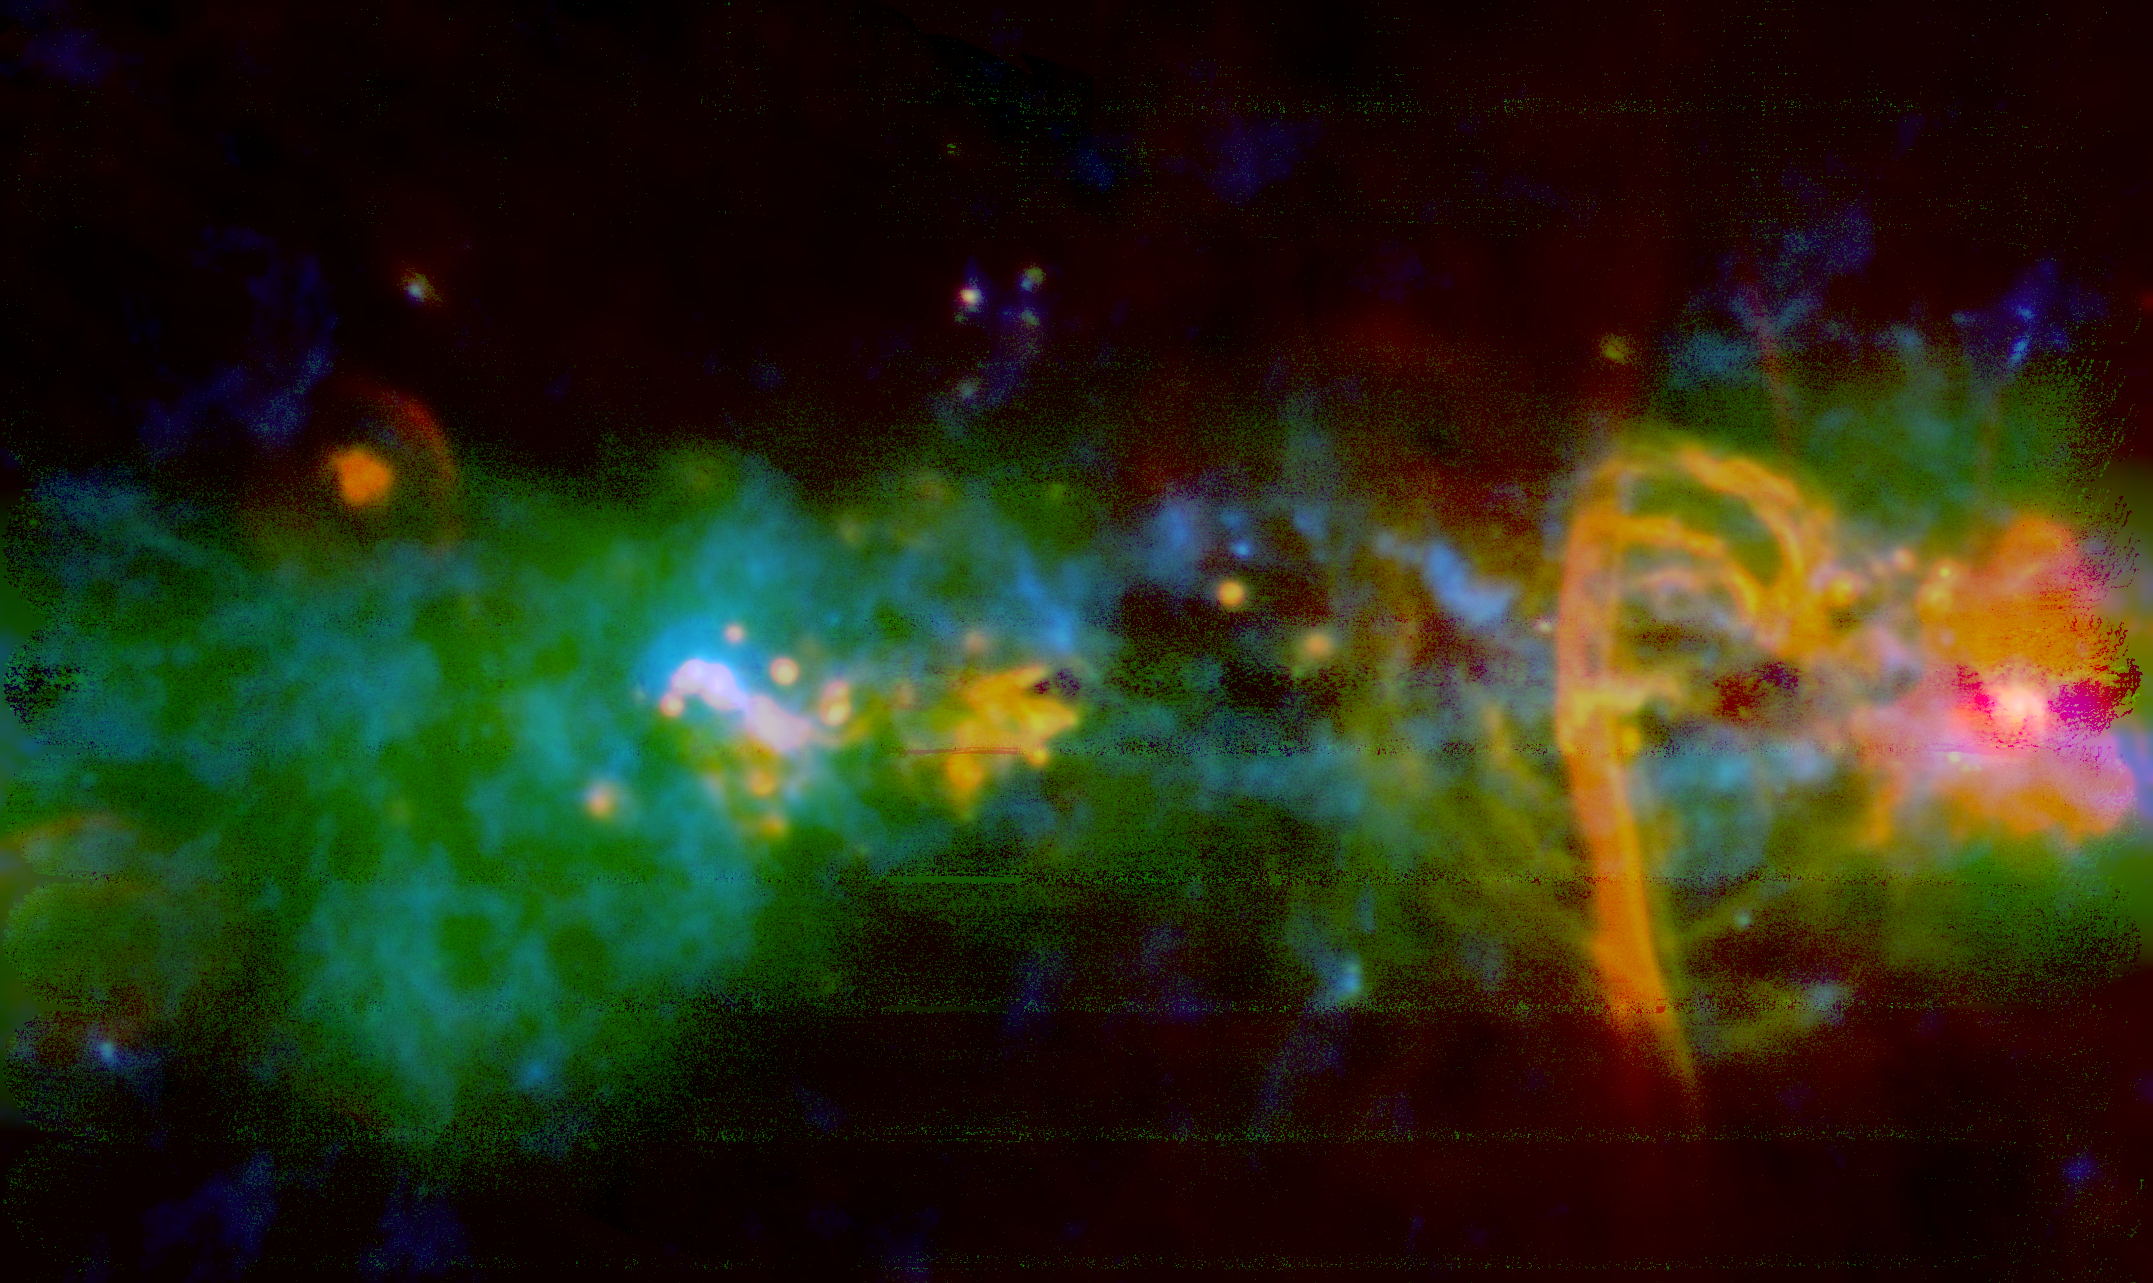
\includegraphics[width=16cm]{SgrB2_RGB_20cm_MGPSplanck_ATLASGAL.png}
%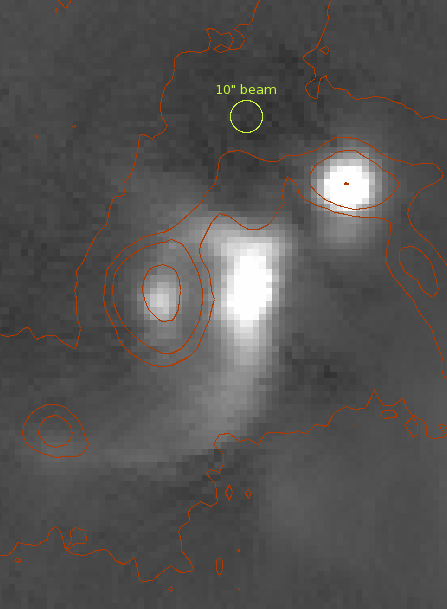
\includegraphics[width=5.5cm]{MUSTANGwithSCUBA450contoursB.png}
\caption{
(top) A color composite of VLA 90 cm (red), \MGPS (green), and JPS 850 \um (blue)
images of the W43 region ($\ell=30\deg$).  The \MGPS data primarily pick up
the ionized gas seen at longer wavelengths, with some contribution from the 
850 \um-bright dust; the inset shows the W43 region in grayscale as seen by
\MGPS.  There are a few sources (e.g., one identified by an arrow) that are strongly detected at 3 mm but not
at 850 \um or 90 cm; these are hypercompact \hii regions that represent
the late stages of accretion in high-mass star formation.
(bottom) VLA 20 cm (red), \MGPS combined with Planck (green), and ATLASGAL
870 \um (blue) composite of the Galactic Center, illustrating the much better
recovery of dust emission at 3 mm in this region and hinting at a change in
dust opacity.
}
\label{fig:figure}
\end{figure}

\clearpage

NOTE: THIS DOCUMENT IS INTENDED TO BE CUT HERE.  Only the first 4 pages are to be submitted.


% \Figure{coverage_gc.pdf}
% {The target regions superposed on an emission map from the BGPS
% \citep{Aguirre2011a,Ginsburg2013a}.  The red boxes represent the approximate
% area to be covered by \MUSTANG.  The labels indicate source names \& distances
% for the massive proto-clusters being targeted.  The observed 1-square-degree
% regions include the entire parent molecular clouds of the massive clumps.  The
% 1-degree size scale is selected because \MUSTANG is very efficient at
% covering maps of this size, and a Galactic plane survey can be carried out with
% the same configuration.  The large maps are essential to include the complete
% molecular clouds, since massive star formation is not isolated to the cluster
% regions.}
% {fig:coverage}{0.3}{0}
% 
% 
% 
% \Figure{rKuVLA_gMUSTANG_bSCUBA450.png}
% {RGB image showing some of the first MUSTANG-1.5 data taken in the Galactic plane toward the W51 star-forming region.  Red is JVLA Ku-band, green is MUSTANG-1.5 (with RMS $\sim10$ mJy, much higher than our target), and blue is SCUBA-2 450um.  In this bright extended HII region, the 3mm emission is dominated by free-free emission, }
% {fig:mustangRGB}{0.25}{0}


%\textbf{Final note:} This is a resubmission of the A-ranked proposal
%GBT/14A-329 (linear rank score 0.82), which was not observed because of instrument delays, and
%GBT/15A-172.  We have addressed the concerns expressed in the latter review.
%Our sources are only observable for a portion of this proposal cycle
%(August-October), so completion may require either receiving
%an A-ranking or a resubmission next cycle.

\clearpage
{\color{red} Bibliographies take space and leaving them out doesn't seem to cause complaints...}
%\begin{multicols}{3}
%\begin{spacing}{0.5}
\footnotesize\raggedright
\noindent 
%\vskip-15pt
%\bibliography{bibdesk}
\bibliography{extracted}
\normalsize
%\vskip-15pt
%\end{spacing}
%\end{multicols}
%\bibliography{bibdesk}


ABSTRACT:
We propose a Galactic Plane survey with MUSTANG.  The 3 mm window observed by
MUSTANG covers the transition region from dust-dominated emission in the
mm/submm to free-free in the cm regime.  An unbiased survey in this window will
allow us to separate these mechanisms by comparing with other existing data
sets.  We will accurately determine dust-based column densities at 8 arcsecond
resolution,  search for extremely dense hypercompact HII (HCHII) regions that
represent a very early stage of high-mass star formation, measure the ionizing
flux emission in dense molecular clouds, and we will measure the
dust emissivity index to search for variations. These data will provide the
highest-resolution column density maps achievable that are robust against
temperature variation and free-free contamination.  A pilot program was
partially (~1/3) completed in semester 18A, with first maps being produced in
Summer 2018, demonstrating the feasibility of a complete Galactic plane survey
with MUSTANG.


% We propose a pilot program for a Galactic Plane survey with MUSTANG.  We will
% survey the most massive proto-clusters in the Galaxy, aiming to accurately
% determine dust-based column densities at 8 arcsecond resolution while searching
% for extremely dense hypercompact HII (HCHII) regions that represent a very
% early stage of high-mass star formation.  We will measure the full SEDs of the
% proto-clusters by combining MUSTANG-2 with SCUBA, SHARC, AzTEC, and SPIRE data in
% order to accurately measure their total dust mass and ionizing flux
% density. These data will place strong constraints on the dust emissivity index,
% allowing for the best possible measurements of dust and gas mass. 
% They will provide the highest-resolution column density maps achievable that
% are robust against temperature variation and free-free contamination.
% We will obtain a unique sample of very young high-mass protostars.  Finally,
% we will demonstrate the combination of GBT MUSTANG data with ALMA continuum
% data, filling in its missing short information.

\end{document}
